\chapter{Introdução Teórica}

\cite{Dias1994}  diz que a Educação Ambiental se caracteriza por
incorporar as dimensões sociais, políticas, econômicas,
culturais, ecológicas e éticas, deixando claro que ao discutir
qualquer problema ambiental é fundamental a consideração
de todos estes aspectos. Segundo este autor, “a maior parte
dos problemas ambientais tem suas raízes na miséria que,
por sua vez, é gerada por políticas e problemas econômicos,
concentradores de riqueza e responsáveis pelo desemprego
e degradação ambiental”.\\

Brasília foi inaugurada em 21 de abril de 1960

De acordo com o \citeonline{CODEPLANSEPLAN2013}

\begin{figure}[h]
    \centering
    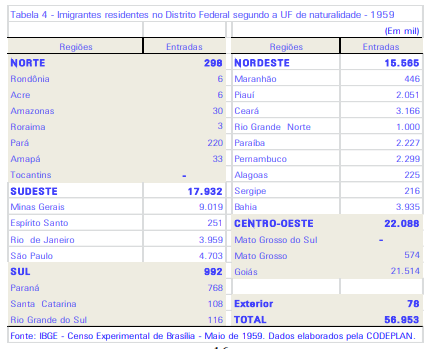
\includegraphics[width=0.7\linewidth]{fig/imigrantes-1959}
    \label{fig:imigrantes-1959}
    \caption{Imigrantes residentes no DF em 1959}
\end{figure}

\lipsum[1-30]

\begin{figure}[h]
    \centering
    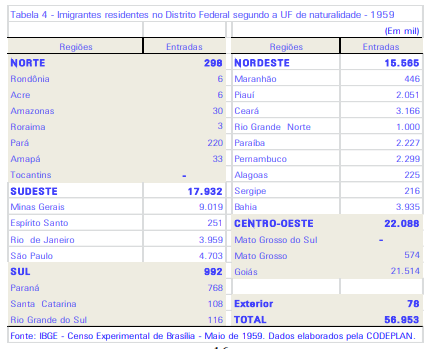
\includegraphics[width=0.7\linewidth]{fig/imigrantes-1959}
    \caption{}
%    \label{fig:imigrantes-1959}
\end{figure}

\begin{figure}[h]
    \centering
    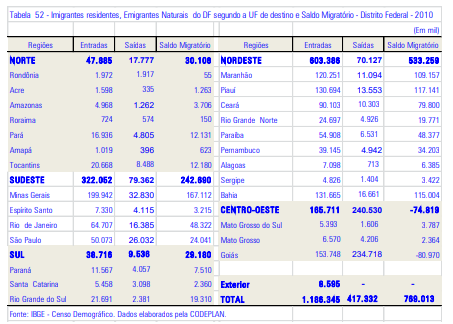
\includegraphics[width=0.7\linewidth]{fig/imigrantes-2010}
    \caption{}
    \label{fig:imigrantes-2010}
\end{figure}
